\ifdefined\XeTeXversion\else\pdfoutput=1\fi
\documentclass[10pt,twocolumn]{article}

\usepackage[margin=0.75in,columnsep=0.24in]{geometry}
\usepackage{amsmath,amssymb}
\usepackage{booktabs}
\usepackage{microtype}
\usepackage{graphicx}
\usepackage{xcolor}
\usepackage{tikz}
\usepackage{xurl}
\usepackage{xspace}
\usepackage[numbers,sort&compress]{natbib}
\usepackage[hidelinks]{hyperref}
\usetikzlibrary{arrows.meta,positioning}

\newcommand{\mgdl}{\ensuremath{\mathrm{mg/dL}}}
\newcommand{\project}{\textsc{GlucoEdge}\xspace}

\title{\project: An Engineering Study of On-Device Five-Class\\
Glucose Trend Forecasting and INT8 Quantization}
\author{Mohamed Menasy\\
Independent Researcher\\
\texttt{mohamedmenasy@gmail.com}}
\date{July 2026}

\begin{document}
\maketitle

\begin{abstract}
We study how INT8 quantization changes a compact glucose trend classifier
and assess whether limited calibration coverage could explain the observed
errors. \project is an open-source Android prototype that
uses 12 five-minute continuous glucose monitor (CGM) readings to predict one
of five rate-of-change classes over the next 15 minutes. A 2,909-parameter
convolutional network was trained
with class-weighted cross-entropy on public Weinstock data prepared by
GlucoBench. On 127,165 aggregate test windows, float LiteRT preserved the
checkpoint's reported accuracy (0.5184) and macro recall (0.5060). Static INT8
quantization using the first 200 validation windows reduced the artifact from
16.95 to 11.70 KiB (31.0\%). Accuracy rose to 0.5866, but macro recall fell to
0.4135: stable-class recall improved while all four directional recalls
declined. Their mean fell from 0.5019 to 0.3537. The recorded input ceiling
near 240 \mgdl\ was below the test maximum of 401 \mgdl. Clipping is therefore
a plausible source of error, but its contribution has not been isolated by
comparing calibration selections. On a Galaxy S22 Ultra, timed inference-path
mean/p95 latencies were
0.334/0.540 ms for float ($n=100$) and 0.484/0.665 ms for INT8 ($n=21$),
excluding softmax and class selection. The unequal replay samples do not
establish a latency benefit. Context-prefix overlap and test-informed class
selection also limit the predictive conclusions. These results describe the
converted models; they do not show whether broader calibration coverage would
recover minority-class recall. \project is a
research demonstration, not a medical device or treatment system.
\end{abstract}

\section{Introduction}

A CGM sampled every five minutes produces 12 observations per hour. These
readings can be used to predict a near-future glucose value, event, or trend
\cite{sergazinov2024glucobench}. Here, we study such predictions for research
purposes; they are not intended to guide treatment.

These targets define different learning problems. Value regression estimates a
future glucose level, event prediction asks whether a glycemic event will occur,
and trend classification assigns a directional rate category. Published studies
also differ in prediction horizon, use of contextual inputs, cohort,
split construction, and metric. Reviews and comparison indices document these
differences. Public benchmarks and cross-dataset experiments help distinguish
performance within a dataset from transfer to another data source
\cite{liu2023systematic,facchinetti2011index,
sergazinov2024glucobench,ghimire2024generalize}. Scores from incompatible
protocols should therefore not be compared directly.

Commercial CGM trend arrows are related but not equivalent targets. They
summarize recent or current glucose direction and rate using device-specific
definitions \cite{pettus2017recommendations,rodacki2021trend}. In contrast,
\project derives each label from the change between the current sample and the
sample 15 minutes later. The arrow-like rate bands provide a compact research
representation, but the future-derived label neither reproduces a manufacturer's
algorithm nor provides a dosing rule.

Deployment raises further questions. Conversion may change a model's outputs,
and the client may need different input handling. Lower precision also does not
guarantee lower latency on a given device. Class imbalance can hide conversion
errors:
accuracy can increase as predictions concentrate on a majority class even while
minority-class recall declines \cite{brodersen2010balanced}.

The motivating research question is: \emph{How does calibration-data coverage
affect minority-class performance and deployment cost in compact glucose trend
classifiers?} Here, coverage refers to the input values and trajectories
represented during quantizer calibration, not calibration of predicted
probabilities. We have results from one trained checkpoint, one calibration
selection, matched float/INT8 evaluations, and one phone. These results show
the observed trade-off and an input-range limitation. They cannot establish
what would change if calibration coverage alone were varied.

This paper follows the model from public CGM preprocessing through conversion
to offline Android replay. It reports:
\begin{itemize}
    \item a segment-aware construction of 12-sample CGM windows and
    future-derived, five-class 15-minute trend labels;
    \item matched evaluation of PyTorch, float LiteRT, and static INT8 LiteRT
    artifacts, showing the opposing changes in accuracy and directional
    recall on the same aggregate test frame;
    \item cross-runtime golden-vector tests and physical-device latency
    observations for an Android \texttt{CompiledModel} implementation; and
    \item an analysis of the observed quantization costs and a possible
    calibration-range explanation, with the comparisons needed to test it.
\end{itemize}

All source code, tests, synthetic replay data, and shipped model artifacts are
available in the project repository.\footnote{\url{https://github.com/mohamedmenasy/GlucoEdge}}

\section{Related Work}

\subsection{Forecasting tasks, horizons, and inputs}

CGM forecasting has expanded from autoregressive value prediction using sensor
history \cite{reifman2007predictive} to recurrent and attention models trained
with CGM and contextual variables \cite{mirshekarian2019lstm}. Recurrent models
have also been used to estimate predictive variance rather than only a point
value \cite{martinsson2020variance}, while convolutional--recurrent models fuse
CGM, insulin, and meal sequences before predicting 30- or 60-minute values
\cite{li2020crnn}. Architecture and input modality change together across these
studies, so their results do not isolate the effect of model family alone.
Cross-dataset evaluation asks a different question: whether a trained model
generalizes when the source dataset, cohort, and collection process change
\cite{ghimire2024generalize}.

Table~\ref{tab:relatedwork} summarizes these design differences. It distinguishes
offline predictive evaluation from reported device execution and omits scores
that would be misleading to compare across protocols.

\subsection{Benchmarks and evaluation protocols}

The split determines what a study can claim about generalization.
Subject-dependent splits evaluate people represented during training;
held-out-participant splits evaluate unseen people within the same dataset.
Cross-dataset evaluation also changes the cohort and data pipeline. GlucoBench
standardizes preprocessing, splits, and baselines across five public datasets
\cite{sergazinov2024glucobench}; experiments across four datasets directly test
changes in data source \cite{ghimire2024generalize}.

\project uses GlucoBench's largest type-1 diabetes cohort, referred to as
Weinstock. Its source study collected blinded CGM from older adults with
long-standing type-1 diabetes \cite{weinstock2016risk}.

Time-series splitting also requires care because nearby and overlapping windows
are dependent. The validity of cross-validation for autoregressive prediction
depends on the residual structure rather than a generic random-split rule
\cite{bergmeir2018crossvalidation}, and leakage can produce answers to a less
demanding problem than the one a study claims to test
\cite{kapoor2023leakage}. Even with a fixed split, training and implementation
choices contribute benchmark variance \cite{bouthillier2021variance}. Results
therefore need to state the participant, temporal, and dataset boundaries used
in evaluation.

\begin{table*}[t]
\centering
\caption{Representative CGM forecasting studies and evaluation scope. Metrics
are not compared across rows because datasets and protocols differ.}
\label{tab:relatedwork}
\small
\resizebox{\textwidth}{!}{%
\begin{tabular}{@{}llllll@{}}
\toprule
Study & Target & Horizon & Inputs & Evaluation scope & Device evidence \\
\midrule
Reifman et al. \cite{reifman2007predictive} & Value & 30 min & CGM & 9 participants & None reported \\
Mirshekarian et al. \cite{mirshekarian2019lstm} & Value & 30/60 min & CGM + context & OhioT1DM/synthetic & None reported \\
Martinsson et al. \cite{martinsson2020variance} & Value + variance & 30/60 min & CGM & OhioT1DM & None reported \\
Li et al. \cite{li2020crnn} & Value & 30/60 min & CGM, insulin, meals & 10 real + 10 simulated & Android timing \\
GlucoBench \cite{sergazinov2024glucobench} & Value trajectory & 60 min & Dataset-dependent & Five public datasets & None reported \\
Ghimire et al. \cite{ghimire2024generalize} & Value & 30/60 min & CGM & Four datasets & None reported \\
\project (this work) & Trend class & 15 min & CGM & Weinstock aggregate test & Android replay timing \\
\bottomrule
\end{tabular}%
}
\end{table*}

\subsection{Trend representations and class imbalance}

Commercial trend arrows summarize recent or current movement using
device-specific categories whose rate bands and look-back intervals differ
\cite{pettus2017recommendations,rodacki2021trend}. A future label instead asks
whether the trajectory after the input window falls, remains stable, or rises.
\project uses these rate bands to define a research target from the sample
15 minutes after the window. It does not reproduce a commercial arrow
algorithm or support treatment decisions.

In the Weinstock windows used here, most labels are stable and faster changes
are relatively rare. Overall accuracy therefore weights the stable class in
proportion to its prevalence. Macro-averaged recall, equivalent to balanced
accuracy for this single-label setting, gives each class equal weight and makes
minority-class degradation visible \cite{brodersen2010balanced}. Macro recall
still does not establish event-level or clinical performance.

\subsection{Edge inference and quantization}

One-dimensional CNNs extract local temporal features with compact feed-forward
networks \cite{kiranyaz2021survey}.

Mobile inference systems can reduce neural-network execution cost through
compression and runtime-specific scheduling \cite{lane2016deepx}, but latency is
a property of the model, runtime, and hardware together. Li et al. reported
Android timing for a glucose forecasting model \cite{li2020crnn}; broader
smartphone and tiny-device benchmarks also measure specified workloads and
platforms because model size alone does not determine speed
\cite{ignatov2019aibenchmark,banbury2021mlperftiny}.

Integer quantization approximates floating-point tensors with discrete values
parameterized by a scale and zero point \cite{jacob2018quantization}. Static
post-training quantization estimates activation ranges from calibration inputs
before conversion \cite{pytorchPT2E2026,googleRepresentativeData}. Low-bit
studies show that clipping, range estimation, and rounding choices can
determine the resulting error \cite{banner2019ptq,nagel2020adaround};
specialized methods have also been proposed to improve post-training accuracy
when calibration sets are small \cite{hubara2021smallcalibration}. These
findings support checking converted outputs and per-class metrics alongside
model size.

\project connects public preprocessing with conversion parity, class-wise
evaluation, and offline replay on one Android device; it does not establish
live-sensor, clinical, or cross-hardware performance.

\section{Problem Formulation}

Let $g_t$ be the CGM value at time $t$, in \mgdl, with observations every five
minutes. The input is
\begin{equation}
    \mathbf{x}_t = [g_{t-55}, g_{t-50}, \ldots, g_t] \in \mathbb{R}^{12}.
\end{equation}
The future rate of change is computed from a point outside the input window:
\begin{equation}
    r_t = \frac{g_{t+15}-g_t}{15}\quad [\mgdl/\mathrm{min}].
\end{equation}
The class $y_t$ is assigned by
\begin{equation}
y_t =
\begin{cases}
\texttt{falling\_fast}, & r_t \leq -2,\\
\texttt{falling},       & -2 < r_t \leq -1,\\
\texttt{stable},        & -1 < r_t < 1,\\
\texttt{rising},        & 1 \leq r_t < 2,\\
\texttt{rising\_fast}, & r_t \geq 2.
\end{cases}
\end{equation}
The 12 readings span 55 elapsed minutes; ``one-hour history'' refers to 12
samples at a five-minute cadence. The history length and 15-minute horizon
are fixed engineering choices for this prototype. The five-class target is a
simplification based on two samples and does not describe the full intervening
trajectory.
The boundaries use rate bands commonly represented by CGM trend arrows, while
collapsing device-specific arrow taxonomies into five classes
\cite{pettus2017recommendations,rodacki2021trend}. No threshold was optimized on
the test labels.

\section{Data and Methods}

\subsection{Dataset and preprocessing}

The experiments use the Weinstock data distributed through GlucoBench. The
source cohort comprised older adults with long-standing type-1 diabetes and
blinded CGM collection \cite{weinstock2016risk}. GlucoBench reports 200
participants before preprocessing and 192 afterwards, with a five-minute
sampling interval \cite{sergazinov2024glucobench}. These counts describe the
benchmark; eligible participant counts for the \project window splits were not
recorded. The configuration used here disables scaling and retains glucose in
raw \mgdl. The formatter interpolates within gaps of at most 45 minutes,
drops segments with fewer than 240 original readings, and tags
each contiguous result with an \texttt{id\_segment}. Because interpolation
precedes windowing, generated values may occur among the inputs or at samples
used to form targets. The configured split holds out 10\% of participants for
an out-of-distribution component and forms temporal validation and test
components from the remaining participants. The formatter combines the test
components into one frame. We report metrics for that aggregate without
separate in- and out-of-distribution results.

Windows are generated independently within each $(\texttt{id},
\texttt{id\_segment})$ group and ordered by time. A window is emitted only when
all 12 input points and the three following horizon steps fit in the same
segment. The stride is one reading, matching an application that updates every
five minutes. This rule prevents a sensor gap or participant boundary from
being treated as a continuous trajectory. Adjacent stride-one windows overlap
heavily and are statistically dependent. The resulting frames yielded 424,462 training,
55,289 validation, and 127,165 aggregate test windows.

Table~\ref{tab:distribution} shows the resulting class imbalance. Both fast
classes exceed 13,000 training windows. A preliminary 20-epoch run obtained
test recalls of 0.5333 and 0.5380 for \texttt{falling\_fast} and
\texttt{rising\_fast}, respectively. Neither met the predeclared condition for
collapsing the classes: fewer than 200 training examples or recall below 0.30.
The deployed model therefore retains all five classes. Test recall informed
this five-versus-three decision, so it must be treated as an exploratory
development choice rather than independent validation.

\begin{table}[t]
\centering
\caption{Window distribution after GlucoBench formatting. Percentages are
within each split.}
\label{tab:distribution}
\small
\begin{tabular}{lrr}
\toprule
Class & Train & Aggregate test \\
\midrule
\texttt{falling\_fast} & 13,260 (3.12\%) & 3,692 (2.90\%) \\
\texttt{falling}       & 40,122 (9.45\%) & 11,387 (8.95\%) \\
\texttt{stable}        & 314,257 (74.04\%) & 95,998 (75.49\%) \\
\texttt{rising}        & 39,428 (9.29\%) & 11,012 (8.66\%) \\
\texttt{rising\_fast} & 17,395 (4.10\%) & 5,076 (3.99\%) \\
\midrule
Total                   & 424,462 & 127,165 \\
\bottomrule
\end{tabular}
\end{table}

\subsection{Model and training}

The \texttt{TrendCNN} accepts tensors of shape $(B,1,12)$. It applies a
one-dimensional convolution from 1 to 24 channels, a second convolution from
24 to 36 channels, ReLU after each layer, adaptive average pooling over time,
and a 36-to-5 linear head. Both convolutions use kernel size 3, stride 1, and
padding 1. The network contains 2,909 trainable parameters.

Training uses inverse-frequency class-weighted cross-entropy, batch size 64,
and Adam with learning rate $10^{-3}$ \cite{kingma2015adam}. The artifact used
for conversion was trained for 20 epochs with PyTorch seed 0
\cite{paszke2019pytorch}. Validation loss was observed after every epoch; there
was no early stopping or test-time selection. Classification reports were
computed with scikit-learn \cite{pedregosa2011scikit}. Because the test
distribution is dominated by \texttt{stable}, macro-averaged recall is the
primary aggregate metric. For single-label multiclass prediction it is the mean
of the five per-class recalls and is equivalent to balanced accuracy
\cite{brodersen2010balanced}.

\begin{figure*}[t]
\centering
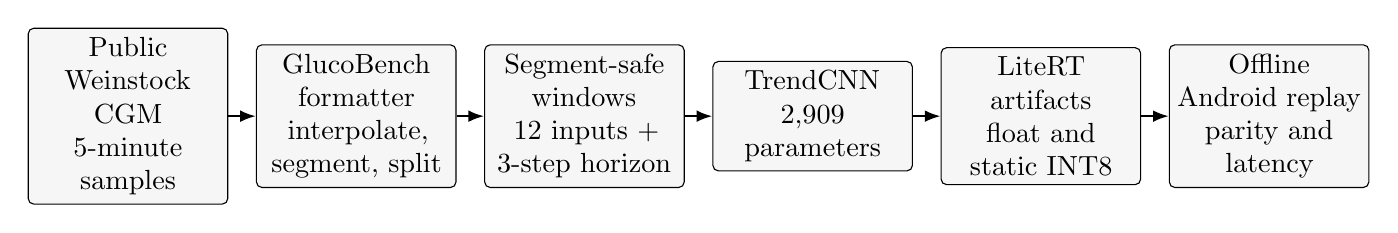
\begin{tikzpicture}[
    node distance=0.35cm,
    box/.style={draw, rounded corners=2pt, align=center, minimum height=1.0cm,
                text width=2.3cm, fill=gray!7},
    arrow/.style={-{Latex[length=2mm]}, thick}
]
\node[box] (data) {Public\\Weinstock CGM\\5-minute samples};
\node[box, right=of data] (format) {GlucoBench formatter\\interpolate, segment, split};
\node[box, right=of format] (windows) {Segment-safe windows\\12 inputs + 3-step horizon};
\node[box, right=of windows] (cnn) {TrendCNN\\2,909\\parameters};
\node[box, right=of cnn] (models) {LiteRT artifacts\\float and static INT8};
\node[box, right=of models] (android) {Offline Android replay\\parity and latency};
\draw[arrow] (data) -- (format);
\draw[arrow] (format) -- (windows);
\draw[arrow] (windows) -- (cnn);
\draw[arrow] (cnn) -- (models);
\draw[arrow] (models) -- (android);
\end{tikzpicture}
\caption{End-to-end \project workflow. Patient data are used locally for
training and evaluation; only model files and a synthetic replay trace are
committed to the Android application.}
\label{fig:pipeline}
\end{figure*}

\section{Conversion and Deployment}

The seed-0 checkpoint was converted with LiteRT Torch. Float conversion uses a
fixed $(1,1,12)$ input signature. INT8 conversion uses PyTorch 2 Export (PT2E),
the quantizer's symmetric configuration helper with
\texttt{is\_per\_channel=True} and \texttt{is\_dynamic=False}, and the first
200 validation windows as calibration inputs. Selection follows the dataset's
participant/segment and time order, with no randomization or attempt to balance
input-range coverage. Because stride-one windows overlap, 200 windows
need not represent 200 independent trajectories. The reported results do not
retain counts of calibration participants or unique readings.

For input scale $s$ and zero point $z$, both clients use the affine form
\begin{equation}
    q = \operatorname{clip}\left(\operatorname{round}(x/s)+z,
    -128,127\right), \qquad \hat{x}=s(q-z).
\end{equation}
Quantization parameters are read from the model metadata rather than hardcoded.
The implementations differ at rounding ties. Python uses
\texttt{numpy.round}, which resolves exact half-way values to even integers,
while Kotlin's \texttt{roundToInt} resolves them toward positive infinity
\cite{numpyRound,kotlinRoundToInt}. The golden-vector tests below check
agreement on selected inputs; they cannot prove that input quantization is
identical for every possible value.

The Kotlin/Jetpack Compose application replays a bundled synthetic trace. A
12-reading ring buffer resets after a cadence gap, mirroring training-time
segment boundaries. Every complete window is classified locally; the merged
Android manifest is tested to ensure it does not request the
\texttt{INTERNET} permission. The float artifact is the default and INT8 can be
selected for comparison.

Real devices use LiteRT 2.1.0 \texttt{CompiledModel} on CPU
\cite{googleLiteRTCompiledModel}. On the tested
Apple-Silicon-hosted Android emulator, native model creation terminated with an
illegal-instruction fault during an ARM SVE feature probe. Because this fault
cannot be caught by Kotlin, emulators are selected before runtime initialization
and use the classic interpreter with XNNPACK disabled. This workaround applies
to the tested environment; it does not establish performance across LiteRT
configurations.

\section{Experimental Protocol}

The aggregate test frame combines temporal and held-out-participant components.
As detailed in Section~\ref{sec:limitations}, the implementation did not exclude
context-prefix rows from eligible target starts. The metrics therefore
describe the shipped model under this protocol and should not be treated as
leakage-free estimates of participant-level generalization.

The same 127,165 aggregate test windows and labels were passed through the
PyTorch checkpoint, float LiteRT model, and INT8 LiteRT model. Accuracy,
per-class recall, and macro recall were computed from each prediction set. A
constant-\texttt{stable} classifier is included to show the effect of class
prevalence. If $n_c$ is class support, $N=\sum_c n_c$, and $R_c$ is class
recall, then
\begin{equation}
    A=\sum_{c=1}^{5}\frac{n_c}{N}R_c,
    \qquad R_{\mathrm{macro}}=\frac{1}{5}\sum_{c=1}^{5}R_c.
\end{equation}
We also summarize the four directional classes, defined here as all classes
except \texttt{stable}, by their unweighted mean recall. This descriptive
summary and the accuracy decomposition below use the existing rounded
per-class reports. Neither required a new training or evaluation run. All
differences refer to the same aggregate windows; no confidence intervals or
significance tests were calculated.

File size is the exact serialized artifact size. Device latency is measured
inside the application's \texttt{classify} method with
\texttt{System.nanoTime}; it includes buffer writes, input quantization when
needed, model execution, and output reading/dequantization. The timer stops
before softmax, class selection, and construction of the returned prediction;
model loading and UI updates are also outside its scope. Measurements were
recorded during replay on a Samsung Galaxy S22 Ultra (SM-S908E, Android 16).
The float statistics use the latest 100 inferences, while the recorded INT8
statistics contain 21 inferences after a model switch. The application reports
p95 as the sorted sample at zero-based index
$\lfloor0.95(n-1)\rfloor$, so these estimates also have different rank
resolution. The timings cover this portion of the inference path during replay.
They measure neither the full classification call nor the kernel alone, and
the runs were not controlled for a benchmark comparison.
Calibration preparation time, peak memory, model-load time, and energy were
not measured.

Cross-runtime parity was tested with 20 synthetic golden windows, four selected
from each float-predicted class and including values above the INT8 input range.
The test also verifies the SHA-256 hash of each bundled artifact. Float logits
must match the Python output within $10^{-5}$; dequantized INT8 outputs are
required to match bit-for-bit because both sides dequantize identical integer
outputs with the same float32 operation.

\section{Results}

\subsection{Predictive performance}

Table~\ref{tab:modelsummary} shows that float LiteRT preserved the checkpoint's
reported classification metrics. The constant majority-class baseline reaches
0.7549 accuracy, higher than either learned model, but its macro recall is only
0.2000. Accuracy alone would therefore favor a model that never predicts a
directional class.

INT8 accuracy increased by 6.82 percentage points relative to float, while
macro recall decreased by 9.25 points. Table~\ref{tab:recall} shows where the
change occurred: recall improved only for \texttt{stable}. It fell for every
minority class. The largest loss was in \texttt{falling\_fast}, whose recall
fell from 0.5119 to 0.1907, a 62.7\% relative reduction. Mean directional
recall fell from 0.5019 to 0.3537, a 14.82-percentage-point decrease derived
from the rounded per-class values.

Weighting each recall change by its class support explains the accuracy gain.
This calculation does not require predicted class frequencies. With the recorded supports,
the stable-class recall gain contributes approximately $+9.84$ percentage
points to accuracy; the four directional losses contribute $-3.03$ points
in total. Summing before rounding yields the reported $+6.82$-point change.
The reported recalls are not enough to reconstruct the full confusion matrix
or predicted class proportions.

\begin{table}[t]
\centering
\caption{Aggregate test metrics. PyTorch and float LiteRT have identical
reported values.}
\label{tab:modelsummary}
\small
\begin{tabular}{lcc}
\toprule
Model & Accuracy & Macro recall \\
\midrule
Constant \texttt{stable} & 0.7549 & 0.2000 \\
PyTorch checkpoint       & 0.5184 & 0.5060 \\
Float LiteRT             & 0.5184 & 0.5060 \\
INT8 LiteRT              & 0.5866 & 0.4135 \\
\bottomrule
\end{tabular}
\end{table}

\begin{table}[t]
\centering
\caption{Per-class recall before and after static INT8 quantization.}
\label{tab:recall}
\small
\begin{tabular}{lrrr}
\toprule
Class & Float & INT8 & Change \\
\midrule
\texttt{falling\_fast} & 0.5119 & 0.1907 & $-0.3212$ \\
\texttt{falling}       & 0.5484 & 0.4306 & $-0.1178$ \\
\texttt{stable}        & 0.5225 & 0.6529 & $+0.1304$ \\
\texttt{rising}        & 0.4761 & 0.3845 & $-0.0916$ \\
\texttt{rising\_fast} & 0.4712 & 0.4090 & $-0.0622$ \\
\midrule
Directional mean & 0.5019 & 0.3537 & $-0.1482$ \\
\bottomrule
\end{tabular}
\end{table}

\subsection{Size, latency, and parity}

Table~\ref{tab:deployment} summarizes deployment measurements. INT8 reduced the
artifact by 5,376 bytes, or 31.0\%. Observed on-device latency did not decrease.
The unequal sample counts prevent a formal comparison, so these measurements
cannot establish a speed advantage for either model.

The July conversion record\footnote{\url{https://github.com/mohamedmenasy/GlucoEdge/blob/513e940/docs/superpowers/specs/2026-07-01-litert-conversion-results.md}}
reports a learned input ceiling near 240 \mgdl,
a test maximum of 401 \mgdl, and saturation in approximately 28\% of test
windows. The figure is approximate: window-level clipping counts, class
breakdowns, and calibration selections were not archived with the paper.
Clipping could contribute to the recall loss, but this record cannot quantify
its contribution for any class. Clipping prevents integer overflow but cannot recover
information outside the representable range.

All three Android instrumentation tests passed on the physical device. The
\texttt{CompiledModel} path loaded both artifact hashes, matched float logits
within $10^{-5}$ on all 20 windows, and matched INT8 dequantized outputs exactly.
The two runtimes therefore agreed on the tested vectors. Differences may still
occur on untested inputs, including exact rounding ties. These tests also
cannot establish whether calibration caused the predictive loss.

\begin{table}[t]
\centering
\caption{Artifact and physical-device observations. Timing ends before
softmax and class selection; sample counts differ by model.}
\label{tab:deployment}
\footnotesize
\begin{tabular}{@{}lrr@{}}
\toprule
Measurement & Float & INT8 \\
\midrule
Artifact size (bytes) & 17,352 & 11,976 \\
Artifact size (KiB) & 16.95 & 11.70 \\
Mean latency (ms) & 0.334 ($n=100$) & 0.484 ($n=21$) \\
p95 latency (ms) & 0.540 & 0.665 \\
Golden vectors passed & 20/20 & 20/20 \\
\bottomrule
\end{tabular}
\end{table}

\section{Discussion}

\subsection{Minority-class performance and deployment cost}

INT8 produced a smaller model file and lower recall for every directional
class. Integer arithmetic often reduces memory and can improve latency for compute-heavy
networks \cite{jacob2018quantization}; here the network is only 2,909 parameters,
so fixed invocation and data-movement costs may dominate the measured path.
Mobile acceleration studies and device benchmarks also show why performance
must be measured for a particular model, runtime, and device
\cite{lane2016deepx,ignatov2019aibenchmark,banbury2021mlperftiny}. The observed
storage saving was a 5.25-KiB file reduction.

The choice of metric changes how this trade-off appears. The stable class
receives approximately three quarters of the weight in accuracy and one fifth
in macro recall. Averaging only the directional recalls makes the
14.82-point loss clear. Float better preserves directional performance in
these results, which is why \project uses it by default. This choice applies
to the measured models and does not rank quantization methods in general.

The 5.25-KiB saving concerns model storage. We did not measure whether it
reduced application size or working memory. The phone ran both models at the
reported latencies, but the uncontrolled workloads and unequal sample counts
prevent a comparison of speed. Calibration preparation time was also not
measured. The results therefore cannot tell us how changing calibration
coverage would affect either preparation cost or runtime cost.

\subsection{What the calibration evidence identifies}

Using 200 calibration windows did not prevent the recorded range mismatch.
Official guidance recommends small representative
subsets of training or validation data to estimate tensor ranges
\cite{googleRepresentativeData,googleLiteRTQuantization}; contiguous,
overlapping validation windows may provide limited diversity. Prior PTQ work
identifies clipping and range estimation as error sources
\cite{banner2019ptq}, optimizes weight rounding
\cite{nagel2020adaround}, and improves quantization with small calibration
sets \cite{hubara2021smallcalibration}. These studies suggest explanations to
test, but do not identify the main source of error in this CGM model.

Broader range coverage is not guaranteed to improve recall. For a fixed
integer code range, increasing the represented interval increases the scale
$s$ and thus the spacing between adjacent representable inputs. Less clipping
therefore comes at the cost of coarser resolution. The future-derived
class depends on a difference between two readings; a high absolute glucose
value does not by itself identify a rapid rise or fall. The aggregate
saturation figure does not tell us whether clipping occurs more often in
any particular directional class.

A follow-up experiment could compare random calibration selection with
selection designed to cover the input range, while keeping model weights,
quantizer, calibration budget, and participant allocation fixed. Selection
must use development inputs without tuning to test labels or test ranges.
Passing quantized and then dequantized inputs through the float model would
measure input-only loss for comparison with full INT8 loss. The remaining
difference could reflect internal quantization and its interaction with input
error. Before this comparison, target overlap must be corrected. Evaluation
should then report each directional recall, paired participant-level
uncertainty, and clipped-input fractions by class. Device measurements would
need identical workloads and controlled repeated runs. These experiments
remain to be done.

The parity tests check agreement for particular inputs and artifact hashes.
Tests of rounding ties, alongside out-of-range values, are needed before
claiming broader arithmetic equivalence. Runtime agreement alone cannot
separate calibration error from other quantization effects. It also does not
validate the labels, cohort split, probability calibration, clinical safety,
or usefulness to a person with diabetes.

\section{Limitations}
\label{sec:limitations}

The results should be read with the following limitations in mind.
\begin{enumerate}
    \item The deployed checkpoint comes from one seed. Training and implementation
    choices can affect benchmark results \cite{bouthillier2021variance}, but we
    did not measure across-seed variability or calculate confidence intervals.
    We also did not evaluate probability calibration, event-level performance, or
    input-dependent temporal baselines beyond the constant-\texttt{stable}
    comparator.
    \item Stride-one windows are overlapping and statistically dependent, so
    their totals are not independent event counts
    \cite{bergmeir2018crossvalidation}. Because GlucoBench interpolates before
    window construction, generated values may occur in model inputs or in
    samples used to form targets. Interpolated inputs can depend on later
    readings, so this retrospective preprocessing may use information that
    would be unavailable in real time. Results are not stratified by interpolation
    status.
    \item GlucoBench adds prefix context to validation and in-distribution test
    frames so sequence models can form initial histories. The current
    \project dataset builder allows every prefix row to start a window and
    does not mask context-only targets. Some aggregate validation/test windows
    can therefore score targets in an adjacent split's context region.
    Using earlier readings as inputs can be legitimate; scoring targets from
    context-only rows introduces a leakage risk and can make evaluation easier
    than intended \cite{kapoor2023leakage}. The reported figures describe the
    built model under this protocol. They are not leakage-free estimates of
    participant-level generalization. A corrected evaluation must mask
    context-only targets, verify disjoint scored participant/segment/time
    keys, and report temporal and held-out-participant components separately.
    \item The aggregate test frame mixes temporal holdouts with participants
    held out by GlucoBench. The source cohort comprised older adults with
    long-standing type-1 diabetes and blinded CGM collection
    \cite{weinstock2016risk}, and no cross-dataset validation was performed.
    We therefore cannot assess transfer across cohorts and collection pipelines
    \cite{ghimire2024generalize}. No participant-stratified,
    demographic, daytime/nighttime, or subgroup results are available.
    \item The five labels are deterministic transformations of a future CGM
    point, not expert annotations. Their thresholds simplify heterogeneous
    commercial trend-arrow conventions. The CGM-only model omits meal, insulin,
    activity, illness, and other covariates.
    \item The INT8 calibration set consists of the first 200 validation windows,
    not a randomized or stratified sample. The observed saturation is therefore
    specific to this conversion protocol. It should not be generalized to INT8.
    Without comparisons of calibration samplers or budgets, we cannot estimate
    the effect of coverage, a dose--response relation, or possible recall recovery.
    \item The phone latency observations use one device, one runtime path, and
    unequal sample counts. Warm-up, temperature, and processor frequency were
    not controlled, and repeated runs were not analyzed. Calibration time,
    model-load time, energy, and
    memory use were not measured. The internal timing excludes softmax and
    class selection.
    \item The application replays synthetic or locally extracted historical
    traces. It does not ingest a live sensor stream and has not undergone
    prospective, external, usability, or clinical validation.
\end{enumerate}

\section{Reproducibility and Ethics}

\subsection{Code, artifacts, and computational record}

The repository contains the training, conversion, benchmark, Android, and test
code. The bundled artifacts were generated from repository commit
\texttt{361148a} with seed 0. Their SHA-256 digests are
\texttt{eb96c7e...08e6} (float) and \texttt{0dc35387...ea29} (INT8); full hashes
are stored beside the assets and asserted by instrumentation tests. Python unit
tests cover label boundaries, segment-aware windows, model shape, conversion
helpers, and synthetic replay behavior. Android unit tests cover replay,
buffering, quantization, latency aggregation, and view-model behavior. A merged-
manifest check enforces the absence of Internet permission.

The conversion requirements record LiteRT Torch 0.9.1, TorchAO 0.17.0, and
Python LiteRT 2.1.5. They also document PyTorch 2.12.1 and NumPy 2.5.0 in the
historical environment, although the top-level requirements pinned older
versions. These records do not constitute a complete environment lock.
PyTorch seed 0 and the formatter's split seed 0 control separate randomization
steps; neither guarantees bitwise retraining across platforms. The artifact
hashes identify the exact models used for replay.

For the September manuscript revision, we reused the July results and
calculated descriptive summaries from the rounded tables. We did not retrain
models, rerun evaluation on the research data, or collect new phone timings.
Machine-readable run reports and the training checkpoint can be regenerated
locally, but are not versioned paper supplements. A fresh run may produce
different numbers from those recorded here.

\subsection{Data availability and research-use scope}

The CGM data are public research data accessed through GlucoBench under the
source dataset's reuse terms \cite{sergazinov2024glucobench}. They are not
committed to the \project repository or the distributed Android build. The
committed replay trace is synthetic. This work makes no diagnosis, monitoring,
treatment, or dosing claim. Its outputs must not be used for medical decisions.
The application displays this restriction in the primary interface.

Code, bundled model files, and synthetic golden vectors are available at
\url{https://github.com/mohamedmenasy/GlucoEdge}; source CGM access is described
by GlucoBench \cite{sergazinov2024glucobench}. The work uses secondary research
data and the prototype has not been studied with newly recruited participants.
We do not claim an institutional ethics determination for this work.

\subsection{AI assistance and author declarations}

OpenAI Codex assisted with language editing during the September manuscript
revision, checked sources, and compared claims with repository code and
recorded results. The draft requires author review.
Funding, competing interests, and CRediT author contributions remain to be
confirmed by the author before submission.

\section{Conclusion}

\project follows a compact five-class CGM trend model from segment-aware
window construction to offline execution on Android. The implementation
documents fixed-shape conversion, integer input handling, artifact provenance,
and cross-runtime parity. Under the recorded calibration protocol, INT8
saved 5.25 KiB while reducing five-class macro recall by 9.25 percentage
points and mean directional recall by 14.82 points. Its higher accuracy
comes from improved stable-class recall and that class's large share of the
test windows. The input-range mismatch makes calibration coverage worth
investigating, but this comparison cannot establish whether broader coverage
would recover recall or how it would affect preparation and deployment cost.
The phone measurements, taken with unequal sample counts, do not establish
an INT8 latency advantage.

These results provide a baseline for a controlled calibration-coverage study.
That study needs corrected target boundaries, comparisons of calibration
selections, repeated seeds, and separate participant-level evaluation.
External validation would follow. This work remains a research prototype.

\bibliographystyle{unsrtnat}
\renewcommand{\bibfont}{\small}
\setlength{\bibsep}{2pt}
\bibliography{references}

\end{document}
